\chapter{Theoretical Framework}

Our goal is to derive a \textit{multiresolution representation of media objects using neural networks}, a concept we will refer to as \textbf{neural media}. To achieve this, we need to understand foundational concepts related to digital media representation, multiresolution theory, and neural networks.

In this context, we define \textbf{media content} as any form of information intended to be consumed, shared, or experienced by an audience. This includes various types of content, such as visual, auditory, and interactive media. These concepts serve to convey ideas, narratives, knowledge, or emotions and they exist in the real world independently of a computer.

A \textbf{media object}, on the other hand, refers to the digital representation of media content, which can be stored, processed, or transmitted electronically. Media objects take various forms depending on the type of data they represent. For instance:

\begin{itemize}
\item \textbf{Images} are digital representations of still pictures, typically stored as 2D arrays of pixel values (e.g., JPEG, PNG).
\item \textbf{Audio} consists of sound recordings represented as waveforms or spectrograms (e.g., MP3, WAV).
\item \textbf{Videos} are sequences of images combined with an audio track (e.g., MP4, AVI).
\item \textbf{3D models} are geometric representations of objects or scenes (e.g., OBJ, STL).
\end{itemize}

When representing real-world media content in a computer, we can apply the \textit{Paradigm of the Four Universes} (\cite{gomes1995}):

\begin{enumerate}
\item \textbf{Physical Universe}: The real-world objects and phenomena we intend to model.
\item \textbf{Mathematical Universe}: The abstract, continuous description of these objects using mathematical formulations.
\item \textbf{Representation Universe}: The discrete approximations of the objects, where continuous signals are sampled and quantized.
\item \textbf{Implementation Universe}: The realm of concrete data structures and algorithms that map the discrete representations into computable forms.
\end{enumerate}


The transition from the physical universe to the mathematical universe involves creating a \textit{mathematical model} of the media content as a continuous signal. Once modeled, the signal is discretized, bringing it into the representation universe. Finally, in the implementation universe, these discrete representations are stored in data structures suitable for computational purposes.

The process of moving from a discrete representation of a signal to its computable form in the implementation universe is called \textbf{encoding}. In this work, we focus on encoding media objects using \textbf{artificial neural networks}. We will show that neural networks can not only approximate the underlying continuous mathematical model of the media content but also provide an efficient representation of its discrete and finite form. Additionally, we will explore how multiresolution theory can be applied within this framework, developing neural network architectures capable of encoding signals at multiple levels of resolution.

In the next sections, we provide an overview of signal processing and deep learning knowledge to familiarize the reader  with the methods employed in our approach.


\section{Media Objects as Signals}

In a broad sense, a \textbf{signal} is a mathematical function that conveys information about a phenomenon. Signals can vary over time, space, or other domains, depending on the nature of the data being represented. Formally, a signal can be defined as a function \( f: \mathcal{D} \to \mathcal{C} \), where:

\begin{itemize}
  \item \( \mathcal{D} \) is the signal natural domain, representing time, space, or another variable.
  \item \( \mathcal{C} \) is the codomain, representing the values or attributes of the signal, such as intensity or color.
\end{itemize}

For example, an audio signal can be described as a function \( f(t): \mathbb{R} \to \mathbb{R} \), where \( t \) represents time and \( f(t) \) provides the amplitude of the sound wave at each moment. Similarly, an image can be interpreted as a two-dimensional signal \( f: U \subset \mathbb{R}^2 \to \mathcal{C} \) that maps spatial coordinates, a subset of the 2D Euclidean space, to color values. 

For an image to be precisely defined, we must provide a mathematical model for color. Typically, $\mathcal{C}$ is a subspace of $\mathbb{R}^3$. For instance, in the \textbf{RGB color model} each point \( (x, y) \) in the image maps to a vector \( (R, G, B) \) representing the intensities of red, green, and blue. Alternatively, in the \textbf{HSV color model}, the color space is parameterized by hue (H), saturation (S), and value (V), which provides a more perceptually intuitive representation of colors. For a detailed discussion on mathematical models for colors, please refer to \cite{ipcgVelho2014}.

A 3D surface can also be interpreted as a signal, specifically as a function that encodes the geometric and spatial properties of the surface. One way to do this is by modeling the 3D object using a function that describes the surface implicitly as the zero level set of a scalar field. An implicit surface can be represented by a function \( f : \mathbb{R}^3 \rightarrow \mathbb{R} \), where for any point \( \mathbf{x} = (x, y, z) \in \mathbb{R}^3 \), the function returns a scalar value that encodes the \textit{signed distance} or some similar measure from the surface. The surface itself is defined as the set of points where the function evaluates to zero:

\[
\mathcal{S} = \{ \mathbf{x} \in \mathbb{R}^3 \mid f(\mathbf{x}) = 0 \}
\]

In this case, \( f(\mathbf{x}) \) is called an \textbf{implicit function}, and the surface is the \textit{zero level set} of this function. Points where \( f(\mathbf{x}) < 0 \) lie inside the surface, and points where \( f(\mathbf{x}) > 0 \) lie outside the surface. For example, a sphere with radius \( r \) centered at the origin can be described by the implicit function:

\[
f(\mathbf{x}) = \|\mathbf{x}\| - r
\]

Interpreting \textbf{media objects} such as audio, images, and 3D models as signals is a natural and powerful approach because it allows us to apply established mathematical frameworks from signal processing. By treating these objects as signals, we can leverage techniques such as sampling, filtering, and reconstruction to model, analyze, and manipulate them.

% ### Graphical Objects as Signals

% Media objects can be modeled mathematically as signals by considering their structure and attributes. Following the formalism of \cite{gomesGraphical1996}, a graphical object \( \mathcal{O} \) is defined as a pair \( (\mathcal{U}, f) \), where:

% \begin{itemize}
%   \item \( \mathcal{U} = \{U_1, \dots, U_m\} \), with each \( U_i \subset \mathbb{R}^n \), is a collection of subsets of a Euclidean space \( \mathbb{R}^n \) that defines the \textit{geometric data set} of the object.
%   \item \( f: U_1 \cup \dots \cup U_m \to \mathbb{R}^p \) is the \textit{attribute function}, which assigns values (such as color, texture, or other physical properties) to each point in the geometric data set.
% \end{itemize}

% In this formalism, the domain \( U = U_1 \cup \dots \cup U_m \) defines the shape of the object, while the attribute function \( f \) assigns the object's properties. This perspective aligns well with interpreting media objects as signals, where the geometric structure corresponds to the domain, and the attributes of the object correspond to the signal values.


% #### Video as Signals

% A video can be viewed as a sequence of images evolving over time, making it a three-dimensional signal. It can be represented as a function \( f(x, y, t): \mathbb{R}^2 \times \mathbb{R} \to \mathcal{C} \), where \( (x, y) \) represents spatial coordinates, \( t \) is the time dimension, and \( \mathcal{C} \) is the color space. Each frame of the video corresponds to a 2D slice of the signal at a particular time.

% \[
% f(x, y, t) = \text{color at pixel } (x, y) \text{ at time } t
% \]

% This interpretation allows us to analyze both spatial and temporal aspects of the video signal, applying techniques such as spatiotemporal filtering, frame interpolation, and video compression.


\section{Overview of Signal Processing Theory}

\subsection{Sampling and Reconstruction}

Due to the finite nature of computational systems, continuous signals and objects must be represented in a discrete form and stored in finite data structures. While certain media objects can be described through continuous mathematical models, such as vector graphics and other parameterized representations, these are less frequently employed for most practical purposes due to computational complexity or dificulty in modeling.

\textbf{Sampling} is the process of converting a continuous signal, such as an analog image or audio waveform, into a discrete sequence of values. One way this is accomplished is by measuring the signal's amplitude at specific intervals uniformly distributed in time and/or space, where the distance between consecutive measurements is known as the \textit{sampling rate}.

Discrete representations are easy to store and map to data structures; however, many operations—such as resizing, rotation, or resampling of the signal—require us to work with the continuous form of the signal. In such cases, the challenge lies in accurately reconstructing the continuous signal from its discrete samples. According to the theory of sampling and reconstruction, this reconstruction can be achieved under certain conditions. Figure \ref{f:sampling-reconstuction} illustrates the uniform sampling and reconstruction of a one-dimensional signal.


\begin{figure}[!h]
  \centering
  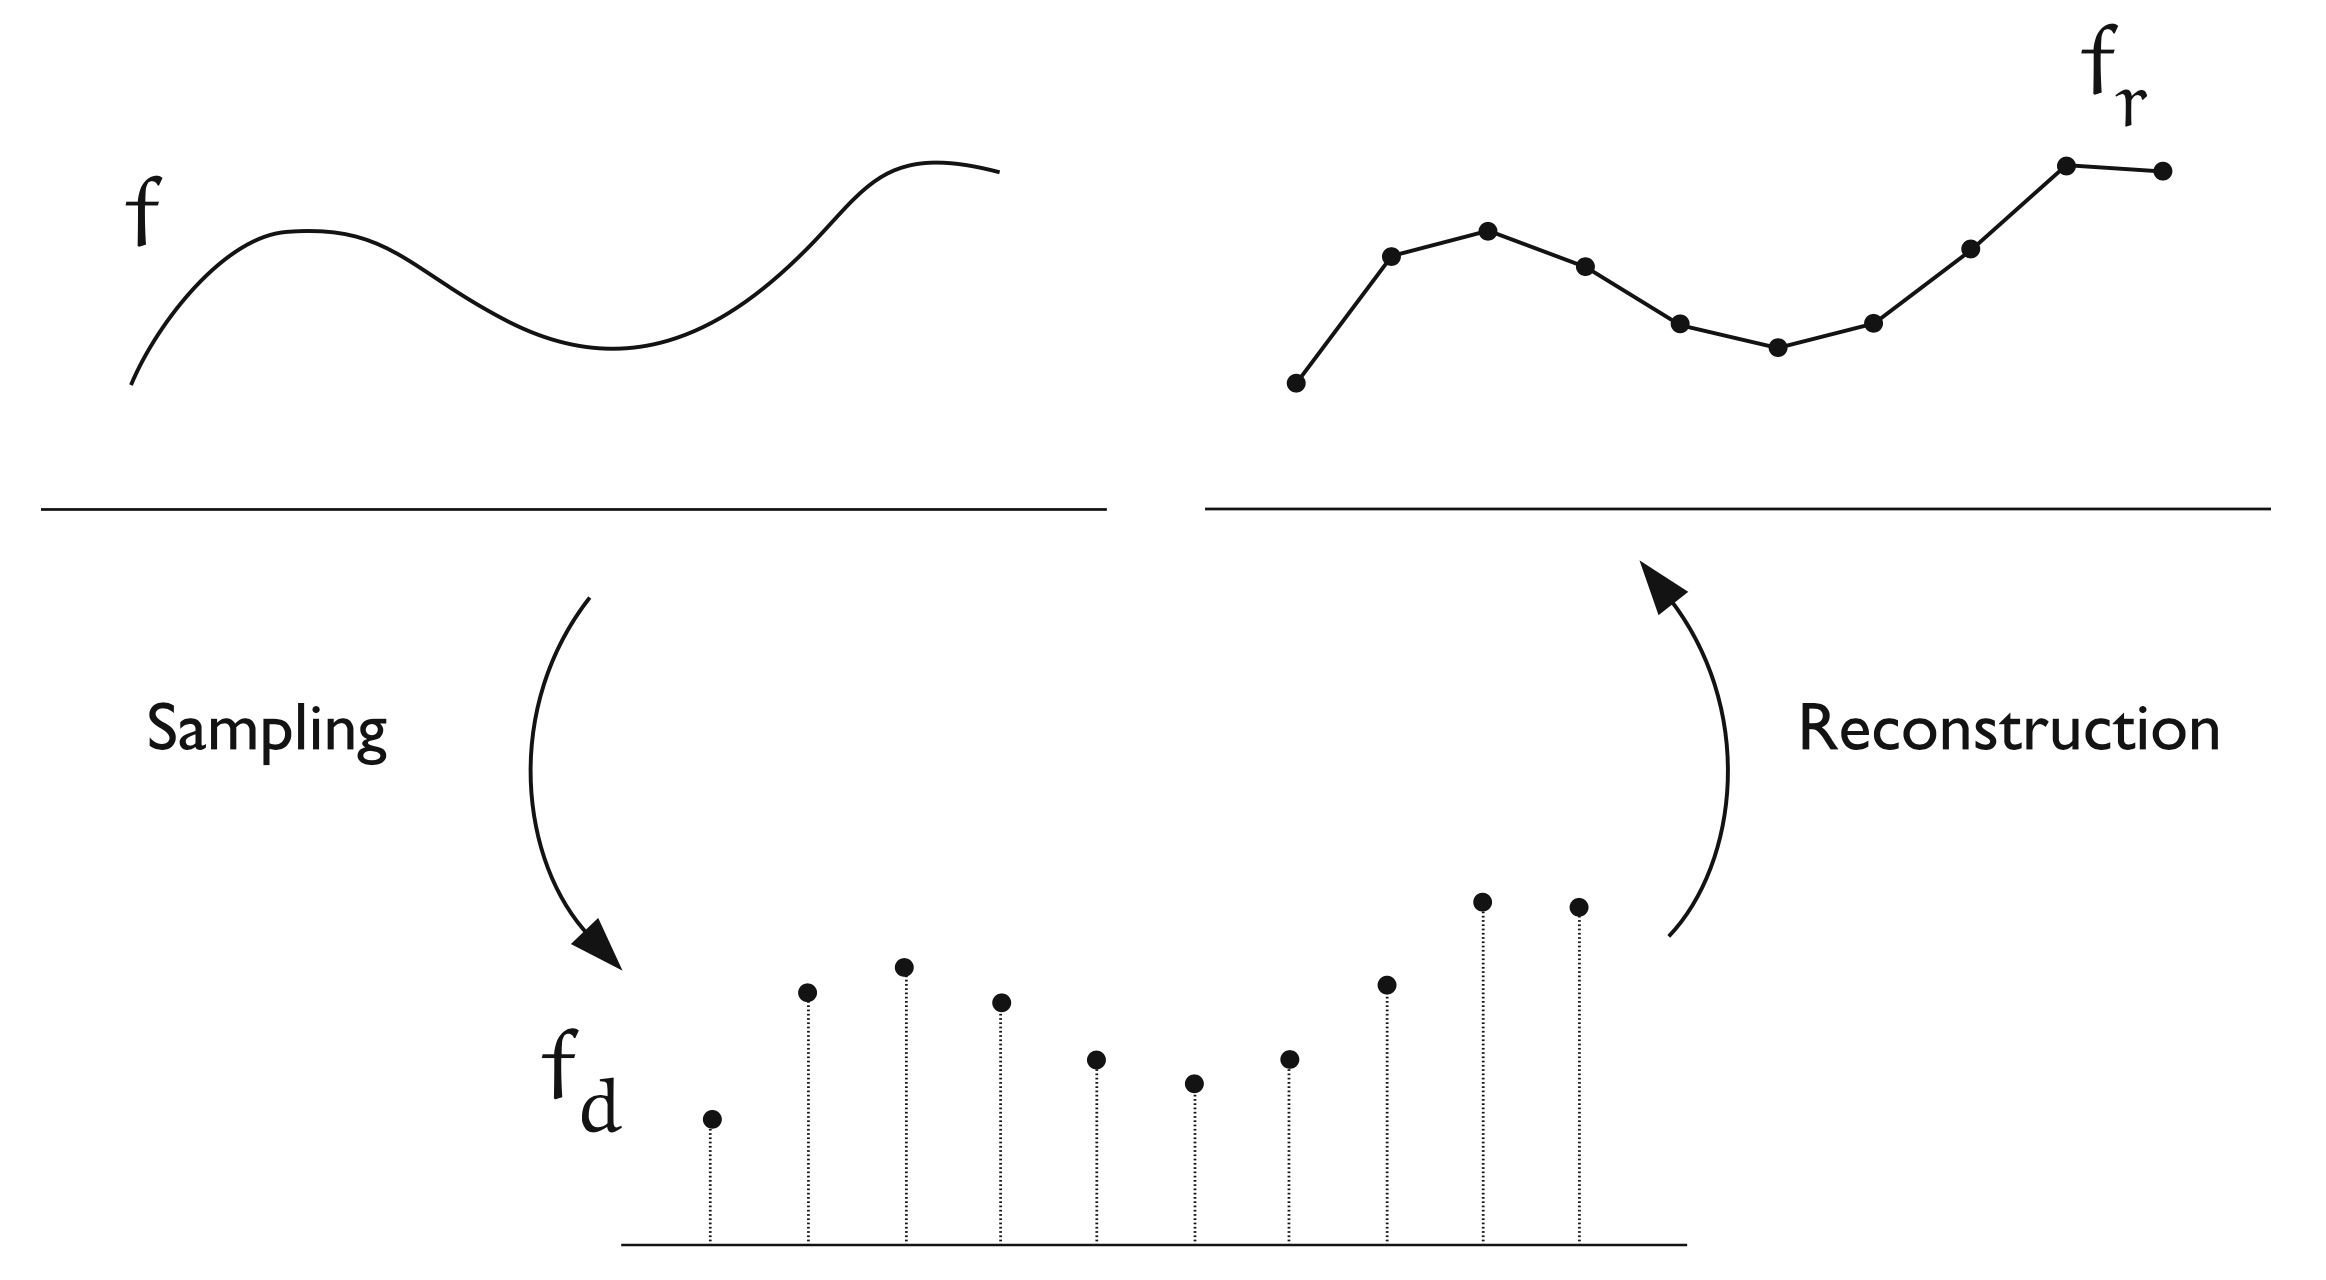
\includegraphics[width=0.85\linewidth]{img/ch2/sampling-reconstruction.png}
  \caption{Illustration of sampling and reconstruction processes.}
  \label{f:sampling-reconstuction}
\end{figure}


One of the fundamental results in this area is the \textbf{Shannon-Nyquist Sampling Theorem} \cite{Shannon1949}. This theorem asserts that a continuous-time, band-limited signal can be perfectly reconstructed from its samples, provided that the sampling rate is at least twice the highest frequency present in the signal. Formally, for a continuous-time signal \( x(t) \) with a maximum frequency component of \( B \) Hz, perfect reconstruction is possible if the sampling frequency \( F_s \) satisfies:
\[
F_s \geq 2B
\]
This critical threshold, \( 2B \), is known as the **Nyquist frequency**.

- \( F_s \): Sampling frequency (in samples per second)
- \( B \): Maximum frequency of the signal (in Hz)

The theorem is central to digital signal processing, as it guarantees that a sufficiently sampled signal retains all the information of its continuous counterpart.

When the sampling frequency falls below the Nyquist limit, \textbf{aliasing} occurs. Aliasing is a form of signal distortion where higher frequency components are misrepresented as lower frequencies in the discrete signal. This distortion results in an inaccurate and misleading reconstruction of the original signal, as illustrated in Figure \ref{f:aliasing-example}.

\begin{figure}[!h]
  \centering
  
\includegraphics[width=0.85\linewidth]{img/placeholder512.png}
  \caption{Illustration of Aliasing.}
  \label{f:aliasing-example}
\end{figure}

The Shannon-Nyquist theorem applies to \textbf{band-limited} signals—those whose frequency content is confined within a finite range. If a signal contains infinite frequency components, no finite sampling rate can fully capture its information. In such cases, even a high sampling rate would still result in aliasing, as the unbounded frequency components would fold into the baseband and distort the signal during reconstruction.

The process of signal reconstruction can be viewed as a form of interpolation. If the sampling adheres to the Nyquist criterion, the continuous signal can be exactly reconstructed using the sinc function as the interpolation kernel. The sinc function is defined as:

\begin{align}
  \text{sinc}(t) = \frac{\sin(\pi t)}{\pi t}
\end{align}

The reconstructed signal is obtained by convolving the discrete samples with the sinc function. In essence, this operation fills in the gaps between sampled points by interpolating based on the sinc kernel. 

**Ideal Interpolation**: The sinc function provides the theoretical basis for perfect interpolation. When applied correctly, it allows for the exact recovery of the original continuous signal from its discrete samples, provided the sampling conditions are met.

However, this ideal reconstruction method is not physically realizable. The sinc function extends to infinity in both directions, making it impractical for real-world implementation. Additionally, the ideal low-pass filter that corresponds to the sinc function features a perfectly sharp cutoff at the Nyquist frequency, which is impossible to achieve due to physical constraints in filtering technology.

In conclusion, while the sinc function and ideal low-pass filter represent theoretical constructs for perfect signal reconstruction, their practical implementation is hindered by real-world limitations. Nonetheless, they serve as benchmarks against which practical signal processing techniques are measured.


% % \red{**Implications for Neural Networks**: Relate these ideas to neural networks and why they struggle to learn high-frequency content.}


\subsection{Frequency Domain Analysis and Fourier Transform}

Any signal can be represented in both its natural domain (such as time or space) and the frequency domain, also known as the spectral domain. The frequency domain provides a powerful framework for analyzing signals by decomposing them into their constituent frequency components. This perspective reveals critical information about the signal's structure, such as its bandwidth, periodicity, and the contribution of different frequencies to the overall signal.

The \textbf{Fourier transform} is the mathematical operation that connects the time or space domain with the frequency domain. It decomposes a signal into a series of sine and cosine waves, each with a specific frequency, amplitude, and phase. For a continuous-time signal \( x(t) \), the Fourier transform \( X(f) \) is defined as:
\[
X(f) = \int_{-\infty}^{\infty} x(t) e^{-j2\pi ft} dt
\]
where:

- \( x(t) \): the time-domain signal,
- \( X(f) \): the frequency-domain representation,
- \( f \): the frequency,
- \( j \): the imaginary unit.

The Fourier transform operates by multiplying the time-domain signal by a complex exponential function for each frequency \( f \) and then integrating the result over all time. This process extracts both the amplitude and phase of each frequency component, revealing the signal's frequency content. By analyzing the frequency spectrum, which consists of the frequencies present in the signal and their associated amplitudes, we can gain insight into the signal's characteristics. 

- **Amplitude**: The amplitude of a frequency component indicates its magnitude or intensity. In the context of audio signals, amplitude corresponds to loudness, while in image processing, it affects brightness or contrast. The amplitude of each frequency component reflects how much that frequency contributes to the overall signal.
  
- **Phase**: The phase represents the initial angle or starting position of the sinusoidal wave at a particular frequency. It determines the relative timing between different frequency components and can affect the overall shape of the signal. Phase shifts can introduce delays or modify the waveform, altering the temporal or spatial structure of the signal.

% % This approach is invaluable in many applications, from audio processing to image analysis and medical imaging, where understanding a signal's frequency content is essential.

The Fourier transform has several forms depending on the nature of the signal. The \textit{continuous Fourier transform} is used for continuous-time signals, while the \textit{discrete Fourier transform} applies to sampled or discrete signals. The \textbf{fast Fourier transform (FFT)} is an efficient algorithm for computing the DFT, enabling real-time signal processing in practical applications.

In the previous section, we discussed how signals are sampled and reconstructed, with particular emphasis on the Shannon-Nyquist sampling theorem and the role of the sinc function in ideal signal reconstruction. The Fourier transform of the sinc function is a rectangular function (Figure \ref{sinc-and-rect}), which highlights a fundamental principle of signal processing: smooth functions in the time domain correspond to compact functions in the frequency domain, and vice versa. The sinc function's Fourier transform being a rectangle in the frequency domain illustrates that it acts as an ideal low-pass filter, passing frequencies within a certain range (the band-limited signal) while cutting off higher frequencies that could lead to aliasing.

\begin{figure}[!h]
  \centering
  
\includegraphics[width=0.85\linewidth]{img/placeholder512.png}
  \caption{Sinc function and its Fourier Transform.}
  \label{f:sinc-and-rect}
\end{figure}

% % The **sinc function**, defined as \( \text{sinc}(t) = \frac{\sin(\pi t)}{\pi t} \), plays a crucial role in both the time and frequency domains. It serves as the ideal interpolation kernel for reconstructing continuous signals from discrete samples, ensuring that no information is lost under perfect conditions. 

The Fourier transform not only allows us to decompose signals into their frequency components but also provides a clear connection between sampling theory and frequency domain analysis. The frequency domain offers an intuitive way to understand the **band-limited nature** of signals: only frequencies below the Nyquist frequency are preserved during sampling. Thus, the Fourier transform gives us the tools to analyze which frequencies are captured and which might cause distortion if undersampled.

% \subsubsection{Inverse Fourier Transform}

The \textbf{inverse Fourier transform} is equally important, as it allows us to reconstruct the original signal from its frequency-domain representation. If we know \( X(f) \), the frequency-domain signal, we can retrieve the time-domain signal \( x(t) \) by applying the inverse Fourier transform:

\[
x(t) = \int_{-\infty}^{\infty} X(f) e^{j2\pi ft} df
\]

This operation restores the original signal by summing all its frequency components (sine and cosine waves) back into the time domain. The inverse Fourier transform provides the foundation for reconstructing signals, just as the sinc function is used in the time domain for ideal interpolation.

Thus, the Fourier transform and its inverse create a bridge between the time and frequency domains, allowing us to switch between these perspectives. When combined with sampling theory, these transformations help us understand how signals can be efficiently represented, manipulated, and reconstructed in both domains.

When signals are sampled, we effectively multiply the original continuous signal by a sequence of Dirac delta functions (impulses). In the frequency domain, this multiplication corresponds to a convolution with a train of impulses, which leads to periodic replicas of the signal's frequency spectrum. This relationship emphasizes the importance of the Nyquist criterion: if the sampling rate is too low (below twice the highest frequency in the signal), these spectral replicas overlap, resulting in aliasing. The Fourier transform enables us to clearly visualize this aliasing effect by showing how undersampling distorts the signal’s frequency content.


% % \red{Visualizing Signals in the Frequency Domain**: Use simple examples (e.g., sine waves) to demonstrate how different frequencies combine to form complex signals.

% % 9. **Stochastic Signals and Noise Models**
% %    - **Introduction to Stochastic Processes**: Briefly explain what stochastic signals are and how they differ from deterministic ones.
% %    - **Perlin Noise and Procedural Patterns**: Use Perlin noise as an example to illustrate how randomness is introduced into signals.
% %    - **Filtering and Noise Removal**: Explain basic techniques for handling noise and filtering in both spatial and spectral domains.

\section{Multiresolution Analysis}

Multiresolution analysis (MRA) offers a hierarchical approach to understanding signals at different levels of detail. By breaking down signals into components that represent varying scales of resolution, MRA helps to capture both global trends and fine details. This technique mimics the way we naturally process visual information, focusing on broader patterns while also perceiving intricate details as needed.

In MRA, signals are decomposed into a coarse approximation, which retains the broader features, and a series of detail coefficients, representing finer, localized features. This approach allows for efficient representation and processing of signals, reducing storage requirements and computational complexity by focusing on the relevant details while discarding less important information.

Multiresolution techniques are widely used in areas such as image processing, signal compression, feature extraction, and wavelet analysis. The following sections provide an overview of two primary methods for multiresolution analysis: pyramids and wavelets.

\subsection{Pyramids: Gaussian and Laplacian}

One of the simplest and most common techniques in MRA is the use of \textit{Gaussian and Laplacian pyramids}. These pyramids represent signals at multiple resolutions, enabling efficient manipulation and analysis across scales.

A \textit{Gaussian pyramid} is built by repeatedly downsampling a signal, typically after applying a low-pass filter to avoid aliasing. At each level, the signal is smoothed using a Gaussian kernel and then reduced in size by subsampling. This results in a pyramid of progressively smaller, coarser versions of the original signal, where each level contains less spatial detail than the previous one.

The mathematical formulation for constructing a Gaussian pyramid is:

\begin{align}
  G_l(x, y) = (G_{l-1}(x, y) * H(x, y)) \downarrow 2
\end{align}

where:
- \( G_l(x, y) \) is the Gaussian pyramid at level \( l \),
- \( H(x, y) \) is a Gaussian low-pass filter, and
- \( \downarrow 2 \) denotes downsampling by a factor of 2.

A \textit{Laplacian pyramid} captures the differences between consecutive levels of the Gaussian pyramid, representing the high-frequency details lost during downsampling. By subtracting the smoothed, downsampled signal from its original form, the Laplacian pyramid isolates these finer details, allowing for a detailed multiscale representation.

The relationship between the Gaussian and Laplacian pyramids is given by:

\begin{align}
  L_l(x, y) = G_{l-1}(x, y) - (G_l(x, y) \uparrow 2 * H(x, y))
\end{align}

where:
- \( L_l(x, y) \) is the Laplacian pyramid at level \( l \),
- \( \uparrow 2 \) denotes upsampling by a factor of 2.

The original signal can be reconstructed from the Laplacian pyramid by iteratively adding the details from each level back to the coarser approximations:

\begin{align}
  G_{l-1}(x, y) = G_l(x, y) \uparrow 2 * H(x, y) + L_l(x, y)  
\end{align}

By progressively adding the finer details back to the lower-resolution versions, the full-resolution signal is restored. In applications such as image compression, storing only the coarse approximation and the detail coefficients leads to efficient data representation.

\subsection{Wavelet Transforms}

While pyramid structures provide a basic form of multiresolution analysis, \textbf{wavelet transforms} offer a more sophisticated and flexible framework. Wavelets differ from pyramids in that they allow for localized, multiresolution analysis in both time (or space) and frequency. This makes them especially useful for signals with transient or localized features.

The key idea behind wavelets is to decompose a signal into a series of \textit{scaled} and \textit{shifted} versions of a fundamental waveform, known as the \textit{mother wavelet}. This process captures both the frequency and location information of the signal components, providing a time-frequency representation that is more adaptive than Fourier-based methods.

In wavelet analysis, a signal is decomposed into approximation coefficients (capturing low-frequency information) and detail coefficients (capturing high-frequency details). This is achieved by convolving the signal with a set of filters: a low-pass filter for approximations and a high-pass filter for details. The decomposition is applied recursively to the approximation coefficients, resulting in a hierarchical, multiresolution representation of the signal.

Mathematically, the wavelet decomposition can be expressed as:

\begin{align}
  A_l = (A_{l-1} * \phi) \downarrow 2, \quad D_l = (A_{l-1} * \psi) \downarrow 2
\end{align}

where:
- \( A_l \) represents the approximation coefficients at level \( l \),
- \( D_l \) represents the detail coefficients,
- \( \phi \) is the scaling function (low-pass filter),
- \( \psi \) is the wavelet function (high-pass filter), and
- \( \downarrow 2 \) denotes downsampling by a factor of 2.

Wavelets naturally offer multiresolution analysis, where larger scales correspond to global features (low-frequency components), and smaller scales capture localized details (high-frequency components). This flexibility allows wavelets to handle signals with varying levels of smoothness or complexity.

The original signal can be reconstructed from its wavelet coefficients by reversing the decomposition process, first upsampling the approximation and detail coefficients, and then applying the inverse filters.

\begin{align}
  A_{l-1} = (A_l \uparrow 2 * \phi) + (D_l \uparrow 2 * \psi)  
\end{align}

This reconstruction process is computationally efficient and forms the basis for many practical applications of wavelets, such as image compression (e.g., JPEG2000), signal denoising, and feature extraction.


\section{Neural Networks}

Artificial Neural networks are computational models inspired by the biological neural networks found in animal brains. These networks consist of interconnected units known as \textbf{artificial neurons}, which simulate the behavior of biological neurons. Each neuron receives inputs, processes them through weighted connections, and produces an output that can be transmitted to other neurons. This architecture allows neural networks to learn complex patterns and relationships within data, making them particularly effective for tasks such as image recognition and natural language processing. In fact, they are universal approximators \red{CITE}.

The fundamental building blocks of a neural network are artificial neurons, which receive inputs represented as real numbers. Each input is associated with a weight that signifies the strength of the connection between neurons. The output of a neuron is calculated as the weighted sum of its inputs plus a bias term, expressed mathematically as:

\[
y = f\left(\sum_{i=1}^{n} w_i x_i + b\right)
\]

where \(y\) is the output, \(w_i\) are the weights, \(x_i\) are the inputs, \(b\) is the bias, and \(f\) is an activation function applied to introduce non-linearity into the model.

Weights are critical parameters that adjust during training to minimize prediction error. Biases allow neurons to shift their activation function, providing additional flexibility in modeling complex relationships. Both weights and biases are updated through optimization algorithms during the training process.

Neural networks learn through a process called \textbf{backpropagation}, which efficiently computes gradients needed for optimization. The learning process involves two main steps: 

\begin{enumerate}
    \item \textbf{Forward Pass}: Inputs are passed through the network to obtain predictions.
    \item \textbf{Backward Pass}: The error between predicted outputs and actual targets is calculated using a loss function (e.g., mean squared error or cross-entropy). The gradients of this error with respect to each weight are computed using the chain rule.
\end{enumerate}

The weights are then updated using an optimization algorithm like \textbf{gradient descent}, which adjusts weights in the direction that minimizes the loss function:

\[
w = w - \eta \nabla L(w)
\]

where \(w\) represents weights, \(\eta\) is the learning rate, and \(\nabla L(w)\) is the gradient of the loss function with respect to weights.

Neural networks can be categorized into \textbf{shallow} and \textbf{deep networks} based on their architecture. A shallow network typically consists of an input layer, one hidden layer, and an output layer. In contrast, deep networks contain multiple hidden layers that enable them to learn hierarchical representations of data. Stacking layers increases the representational power of the network; each additional layer allows the model to capture more complex features from the input data.

In the context of neural networks, \textbf{capacity} refers to the ability of a model to fit a wide variety of functions. It is determined by the architecture of the network, including the number of layers and the number of neurons within those layers. A network with high capacity can learn complex patterns in data, while a network with low capacity may struggle to capture the underlying relationships. The capacity of a neural network is closely linked to its \textbf{expressive power}—the range of functions it can approximate. For instance, a deep neural network with many hidden layers and neurons can represent more intricate functions than a shallow network. However, this increased capacity comes with trade-offs, particularly concerning generalization. A highly expressive model might overfit the training data, learning patterns that do not generalize well to new, unseen data, thus requiring regularization techniques to manage this balance.


Activation functions play a crucial role in determining the output of each neuron by introducing non-linearity into the network. Common activation functions include:

\begin{itemize}
    \item \textbf{Sigmoid}: Maps outputs to a range between 0 and 1.
    \[
    f(x) = \frac{1}{1 + e^{-x}}
    \]
    
    \item \textbf{Hyperbolic Tangent (tanh)}: Maps outputs to a range between -1 and 1.
    \[
    f(x) = \tanh(x) = \frac{e^x - e^{-x}}{e^x + e^{-x}}
    \]
    
    \item \textbf{Rectified Linear Unit (ReLU)}: Outputs zero for negative inputs and linear for positive inputs.
    \[
    f(x) = \max(0, x)
    \]
\end{itemize}

The choice of activation function can significantly impact network performance and convergence during training.

% ---

\subsection{Overfitting and Underfitting}

In the context of neural networks, two important challenges are **overfitting** and **underfitting**. These issues arise from how well the model's capacity aligns with the complexity of the data, and they are closely related to how the model performs on the training set versus unseen test data.

**Underfitting** occurs when the model is too simplistic and lacks the capacity to learn the underlying patterns in the data. This typically happens when the network has too few layers or neurons, preventing it from capturing the complexities within the dataset. As a result, the model fails to perform well on both the training data and the test data, as it cannot even identify the basic trends present in the data. An underfitted model is characterized by poor performance across the board.

On the other hand, **overfitting** happens when the model has excessive capacity, allowing it to memorize the training data instead of generalizing from it. While the model might achieve very low error on the training set, it struggles to handle new, unseen data. This occurs because the overfitted model learns specific details and noise in the training data that don't generalize to broader trends in other datasets. Overfitting leads to a situation where the model's performance on the training data is excellent, but its performance on test data is significantly worse.

Mathematically, these two issues can be observed through the behavior of the loss function. In the case of underfitting, both training loss and validation loss remain high, indicating that the model is not capturing enough of the underlying structure of the data:

\[
\text{High training loss and high validation loss:} \quad L_{\text{train}} \gg 0 \quad \text{and} \quad L_{\text{val}} \gg L_{\text{train}}
\]

For overfitting, the training loss becomes very low, but the validation loss is much higher, reflecting the model's poor generalization to new data:

\[
\text{Low training loss and high validation loss:} \quad L_{\text{train}} \approx 0 \quad \text{and} \quad L_{\text{val}} \gg L_{\text{train}}
\]

To address these challenges, it is essential to find a balance between a model's capacity and its ability to generalize. Several techniques are commonly used to combat overfitting, such as regularization, dropout, and early stopping:

- **Regularization** (e.g., L1 or L2) adds a penalty term to the loss function, discouraging overly complex models by constraining the weights. This helps to reduce overfitting by preventing the model from becoming too specialized to the training data.
  
- **Dropout** involves randomly deactivating a portion of the neurons during training. This technique prevents neurons from relying too heavily on one another, forcing the network to learn more robust features that generalize better.
  
- **Early stopping** monitors the performance of the model on validation data during training and stops the process when performance on the validation set begins to deteriorate, thereby preventing overfitting.

Ultimately, understanding how to manage capacity is crucial in designing neural networks that can learn effectively from training data while also generalizing well to new examples. Achieving the right balance between underfitting and overfitting is essential in many fields, such as computer vision and signal processing, where the accuracy of predictions on unseen data is vital for practical applications.

% ---

\subsection{Coordinate-Based Neural Networks and Implicit Neural Representations}

Coordinate-based neural networks represent a breakthrough in how data is modeled and encoded, especially in spatial domains like images and signals. The central concept is to use neural networks to express data as a continuous function of spatial coordinates. By doing this, various types of signals—such as 2D images or 3D shapes—can be represented by mapping spatial coordinates directly to the corresponding output values, like pixel colors or spatial features.

**Implicit Neural Representations (INRs)** are a specific realization of this idea. Unlike traditional methods that rely on discrete grids (e.g., pixel arrays for images or voxel grids for 3D geometries), INRs treat signals as continuous functions. Rather than storing values at fixed, discrete points, an implicit representation defines a function:

\[
f: \mathbb{R}^n \to \mathbb{R}^m
\]

This function maps any coordinate from an \(n\)-dimensional input space to a corresponding \(m\)-dimensional output value. For instance, in the case of a 2D image, an INR would take a coordinate \((x, y)\) as input and return the RGB color value at that point:

\[
\text{Color} = f(x, y) = (R, G, B)
\]

The advantage of this continuous representation is its flexibility—it is not restricted to any specific spatial resolution. In theory, INRs can achieve infinite resolution, meaning they can be sampled at any desired level of detail without the limitations of traditional discrete grids. This is particularly useful for applications like **super-resolution imaging** or working with high-dimensional datasets.

Furthermore, INRs offer **efficient memory usage**. The memory required to store an implicit representation scales with the complexity of the signal rather than its spatial resolution. For complex datasets, this efficiency is crucial because traditional methods might demand excessive storage, especially when handling high-resolution data.

The impact of implicit neural representations extends far beyond storage optimization. INRs are being utilized in several advanced applications in fields like computer graphics and computer vision:

1. **3D Shape Representation**: INRs can outperform traditional 3D shape representations such as meshes or point clouds. By learning continuous functions over geometric shapes, they allow for seamless deep learning-based modeling of shape priors.

2. **Signal Reconstruction**: INRs can be used to reconstruct missing or incomplete data in signals. For example, given a sparse set of image pixels or audio data points, the learned function can fill in the gaps, making INRs particularly valuable in scenarios where the input data is noisy or incomplete.

3. **Solving Partial Differential Equations (PDEs)**: Some architectures, like **Sinusoidal Representation Networks (SIRENs)**, leverage periodic activation functions such as sine functions. This choice of activations enhances the network’s ability to model complex signals, including their derivatives, making SIRENs especially suitable for solving boundary value problems associated with PDEs. The periodic nature of the activations provides an ideal framework for capturing the oscillatory behavior of solutions to such equations.

Thus, coordinate-based neural networks and implicit neural representations represent a paradigm shift in how we approach and process spatial data. By conceptualizing signals as continuous functions instead of discrete samples, these models provide enhanced flexibility, efficiency, and power in representing complex datasets. As research in this area continues to advance, these approaches are likely to drive further innovations across a range of applications, from computer vision to graphics and beyond.

% % Citations:
% % [1] https://github.com/vsitzmann/awesome-implicit-representations
% % [2] https://www.vincentsitzmann.com/siren/
% % [3] https://www.reddit.com/r/MLQuestions/comments/qta8v6/could_someone_explain_what_an_implicit_neural/
% % [4] https://en.wikipedia.org/wiki/Neural_network_(machine_learning)
% % [5] https://aws.amazon.com/what-is/neural-network/
% % [6] https://www.science-on-stage.eu/machine-learning/neurons
% % [7] https://eitca.org/artificial-intelligence/eitc-ai-dltf-deep-learning-with-tensorflow/introduction-eitc-ai-dltf-deep-learning-with-tensorflow/introduction-to-deep-learning-with-neural-networks-and-tensorflow/examination-review-introduction-to-deep-learning-with-neural-networks-and-tensorflow/what-are-the-key-components-of-a-neural-network-and-what-is-their-role/
% % [8] https://en.wikipedia.org/wiki/Artificial_neuron



\subsection{Sinusoidal Neural Networks}

Sinusoidal neural networks leverage sine functions as activation functions, offering a powerful way to model signals with intricate details. The motivation for using sine functions lies in their ability to capture fine variations in data, making them particularly well-suited for representing high-frequency components of signals. In contrast to conventional neural networks that use activation functions like ReLU or sigmoid, sinusoidal networks are designed to approximate complex signals more naturally, especially those characterized by oscillations and periodic patterns.

The use of sine functions allows sinusoidal neural networks to represent signals in both the **spatial** and **frequency** domains. Signals, especially those in fields such as audio, image processing, and computer graphics, often contain fine structures that require high-frequency components for accurate representation. A sinusoidal activation function, defined as:

\[
\sigma(x) = \sin(x)
\]

is inherently capable of generating oscillations. These oscillations enable the network to capture fine variations in data, something that traditional activations might struggle with. This characteristic makes sinusoidal neural networks ideal for tasks where precision at smaller scales is critical, such as super-resolution, texture generation, or even physics simulations.

The relationship between sinusoidal networks and the **frequency domain** is central to understanding their expressive power. In signal processing, the **Fourier series** is a method for expressing a periodic function as a sum of sine and cosine terms, each associated with a specific frequency. A signal \(f(x)\) can be decomposed into a sum of sinusoids as:

\[
f(x) = a_0 + \sum_{n=1}^{\infty} \left( a_n \cos(n x) + b_n \sin(n x) \right)
\]

This decomposition reveals that any periodic signal can be described as a combination of sinusoids of different frequencies. By using sine functions as activations, sinusoidal neural networks can directly represent the frequency components of a signal, offering the ability to capture both low-frequency (coarse) and high-frequency (fine) details. This is particularly useful when modeling signals that vary at multiple scales, as the network can flexibly adapt to different frequency ranges.

**Sinusoidal Representation Networks (SIREN)** are a specific type of neural network that employ sine functions as their core activations. Introduced as an alternative to traditional architectures, SIRENs have shown significant advantages in representing complex signals, particularly in the context of continuous signals such as images, 3D shapes, and physical fields.

A SIREN architecture typically defines each layer of the network as:

\[
y = \sin(Wx + b)
\]

where \(W\) represents the weight matrix, \(x\) is the input, and \(b\) is the bias term. The sine activation allows the network to approximate high-frequency components, which is especially beneficial for tasks like **implicit neural representation** (as discussed previously) and **solving partial differential equations (PDEs)**.

% Advantages of SIREN

% 1. **Modeling Fine Details**: SIRENs excel at capturing fine details and sharp transitions in signals due to the periodic nature of sine functions. This makes them highly effective in applications such as super-resolution imaging, surface reconstruction, and neural rendering.

% 2. **Smooth Representations**: The continuous nature of the sine function ensures that the output of SIRENs is inherently smooth. This property is particularly useful in applications where smoothness and differentiability of the output are required, such as modeling surfaces or fields in 3D space.

% 3. **Efficient Frequency Control**: SIRENs can naturally control the frequency of their output, allowing them to capture both coarse structures and intricate high-frequency details. This multi-resolution capability is a key advantage over conventional neural networks, which may require additional architectural components (e.g., skip connections) to handle multi-scale data effectively.

% Challenges of SIREN

% While SIRENs offer substantial benefits, they also present some unique challenges:

% 1. **Training Stability**: The use of sine activations can lead to instabilities during training, particularly when initializing the weights. If not properly initialized, the network may struggle to converge or produce overly oscillatory outputs. To address this, specific weight initialization strategies, such as **periodic weight scaling**, are often required.

% 2. **Generalization to Low Frequencies**: While SIRENs excel at high-frequency signal approximation, they may struggle to represent low-frequency components effectively. This issue arises because the network is more naturally attuned to oscillatory patterns, which can lead to difficulties when modeling smoother, broader trends in the data.

% 3. **Complexity of Derivatives**: Another challenge comes from the fact that, while sine functions are smooth and differentiable, the resulting derivatives may be complex to compute efficiently for certain high-dimensional tasks, such as solving higher-order PDEs.

% Conclusion

% Sinusoidal neural networks, and particularly SIRENs, represent a powerful framework for modeling signals that contain intricate, high-frequency components. By leveraging sine functions as activations, these networks can capture fine details that are often missed by traditional architectures. While they offer distinct advantages in precision and smoothness, their unique challenges—such as training instability and generalization to low-frequency signals—require careful consideration when applied in practice. Despite these challenges, SIRENs continue to push the boundaries of neural network-based representations in fields like computer vision, graphics, and scientific computing.


% \subsection{Sinusoidal Neural Networks}

% Sinusoidal neural networks, particularly exemplified by **Sinusoidal Representation Networks (SIRENs)**, utilize sine functions as activation functions to effectively model complex signals. The choice of sine functions is grounded in their unique properties that allow these networks to capture fine details and represent intricate spatial patterns. Unlike traditional activation functions like ReLU or tanh, sine functions are periodic and smooth, which is crucial for modeling signals that exhibit oscillatory behavior or require high-frequency detail.

% #### Capturing Fine Details

% The periodic nature of sine functions enables sinusoidal networks to approximate signals with high fidelity. This capability is particularly beneficial in applications involving natural signals, such as images and audio, where fine details are essential for accurate representation. The smoothness of sine functions allows these networks to maintain continuity and differentiability, which is vital when modeling physical phenomena governed by partial differential equations (PDEs). 

% By employing sine activations, SIRENs can effectively represent a signal's derivatives, which are often critical in understanding the underlying dynamics of the data being modeled. This characteristic makes them suitable for solving boundary value problems, such as the Poisson equation or the Helmholtz equation, where precise control over spatial and temporal derivatives is necessary.

% #### Frequency Domain Representation

% The link between sinusoidal activations and Fourier series further elucidates their effectiveness in signal representation. Fourier series express periodic functions as sums of sine and cosine terms, allowing for the decomposition of signals into their frequency components. In this context, sinusoidal neural networks can be viewed as approximating a function through a harmonic sum:

% $$
% f(x) = \sum_{n=0}^{N} a_n \sin(b_n x + \phi_n)
% $$

% where $$a_n$$, $$b_n$$, and $$\phi_n$$ represent the amplitude, frequency, and phase shift of each harmonic component. This formulation highlights how SIRENs can leverage the properties of sine functions to capture both low-frequency trends and high-frequency details in a unified framework.

% #### Overview of Sinusoidal Representation Networks (SIREN)

% SIRENs are designed specifically to harness the advantages of sinusoidal activations for implicit neural representations. They consist of multiple layers where each layer applies a sine activation function to its outputs. This architecture allows SIRENs to model complex natural signals while maintaining smoothness and continuity across the representation.

% One of the key advantages of SIRENs is their ability to represent signals at varying resolutions without being constrained by traditional grid-based representations. This flexibility enables them to achieve high fidelity in tasks such as image synthesis, 3D shape representation, and audio signal modeling. Additionally, SIRENs have demonstrated superior performance in reconstructing signals from sparse data compared to conventional neural architectures.

% However, training SIRENs presents unique challenges. The periodic nature of sine functions can lead to difficulties in convergence during optimization due to the presence of multiple local minima in the loss landscape. To address this issue, effective initialization schemes are crucial for ensuring stability during training. These schemes help guide the optimization process toward regions of the parameter space that facilitate learning.

% In summary, sinusoidal neural networks leverage the properties of sine functions to provide robust representations of complex signals. Their ability to capture fine details through smoothness and periodicity makes them particularly well-suited for applications that require high precision in modeling physical phenomena. As research continues to advance in this area, SIRENs stand out as a powerful tool for bridging the gap between spatial and frequency domain representations in various fields such as computer graphics, audio processing, and beyond.

% Citations:
% [1] https://docs.siml.ai/creating-a-simulator/neural-network-node/sinusoidal-representation-network
% [2] https://arxiv.org/abs/2212.01833
% [3] https://www.vincentsitzmann.com/siren/
% [4] https://openreview.net/pdf?id=Sks3zF9eg
% [5] https://arxiv.org/abs/2109.09338v2
% [6] https://www.visgraf.impa.br/Data/RefBib/PS_PDF/mrnet-cag-2023/MRNet_CAG-2023.pdf
% [7] https://towardsdatascience.com/sinusoidal-neural-networks-for-digit-classification-bd2b14e57ad8
% [8] https://www.reddit.com/r/MLQuestions/comments/qta8v6/could_someone_explain_what_an_implicit_neural/